% Author: Mathias Hablützel

\section{Berechnung von Segelgeschwindigkeit anhand der Windfelder}
Die in Abschnitt \ref{s:windfields} eingelesenen Windfelder werden nun für die
Berechnung der Segelgeschwindigkeit verwendet. Gegen sind der
Windangriffswinkel auf das Schiff durch die Windvektoren von Punkt $A$ nach
$B$, die Segelrichtung ist damit auch bekannt.

% TODO: Skizze zeichnen mit Punkt A -> B, Segelboot, Windvektoren
 
\subsection{Geschwindigkeit am Ausgangspunkt}
Da es bekannt ist zu welcher Zeit man am Ausgangspunkt $A$ ist, weiss man auch
welcher Windvektor existiert (der sich ja mit der Zeit verändert). Somit lässt
sich die Geschwindigkeit des Bootes am Ausgangspunkt berechnen.

\subsection{Geschwindigkeit am Zielpunkt}
Hier besteht das Problem, dass es nicht bekannt ist, wann das Boot am Punkt $B$
ankommt, die Ankunftszeit hängt vom Windvektor $v_{1}$ in Punkt $A$ zur Zeit
$t_{1}$ und vom Windvektor $v_{2}$ in Punkt $B$ zur Zeit $t_{2}$ ab. $t_{2}$
ist unbekannt und folglich ist $v_{2}$ auch nicht bekannt (nur dessen Position
ist im Voraus bekannt).

Also muss in einem ersten Schritt die Ankunftszeit approximiert werden.  Wir
könnten die Euler'sche Regression verwenden, allerdings besteht hier das
Problem, dass der Algorithmus nicht zwingend die beste Lösung findet und über
eine unterschiedlich lange Laufzeit verfügt. Daher erschien ein zweischrittiges
Verfahren für eine Teilapproximation vernünftig, welches in linearer Zeit
ausgeführt werden kann.

\subsection{Berechnung der Ankunftszeit}
Vom Startpunkt $A$ ist die Uhrzeit, die Position und somit der Windvektor
bekannt. Daraus kann die Geschwindigkeit des Segelbootes bestimmt werden
(ausgehend von Punkt $A$). Diese Geschwindigkeit wird nun für die gesamte
Distanz angenommen und daraus resultiert eine ungefähre Ankunftszeit. Wir
nehmen hier an, dass das Windfeld zu einem späteren Zeitpunkt nicht so stark
ändert, dass unsere Berechnungen zu stark von einem vernünftigen Wert abweicht,
unter anderem weil dies der Natur von Windfeldern widersprechen würde.
Ausgenommen sind Extremsituationen wie Windhosen oder Tornados. Aber in solchen
Situationen wäre das Segeln auch nicht vernünftig.

\subsection{Kurs (Track)}
Die Geschwindigkeit des Segelschiffes hängt einerseits von der Intensität des Windes und andererseits von der Einfallswinkel des Windvektors ab. Damit der Einfallswinkel des Windvektors berechnet werden kann, muss bekannt sein, in welche Richtung das Segelschiff segelt. Die Berechnung des Kurses findet wie folgt statt: Zuerst wird ein Kreuzprodukt der zwei Vektoren vom Ursprung  \(\overrightarrow{A}\) und \(\overrightarrow{B}\) brerechnet. Das Resultat entspricht dann der Normalenvektor \(\overrightarrow{N}\), welche senkrecht zu der aufgespalteten Ebene von \(\overrightarrow{A}\) und \(\overrightarrow{B}\) steht. Danach wird wiederum ein Kreuzprodukt berechnet, diesmal aber vom Vektor \(\overrightarrow{A}\) und dem Normalenvektor \(\overrightarrow{N}\). Dies ergibt als Resultat die Richtung des Segelschiffes. Da dieser Vektor aber 3-dimensional ist, muss sie auf die lokale Tangentialebene (\(\overrightarrow{e_{\theta}}\), \(\overrightarrow{e_{\phi}}\)) des Punktes $A$ projiziert werden, damit wir ein 2-dimensionales Vektor kriegen. \\
Die grafische Darstellung dieser Berechnung sieht wie folgt aus:
\begin{figure}[h!]
\centering
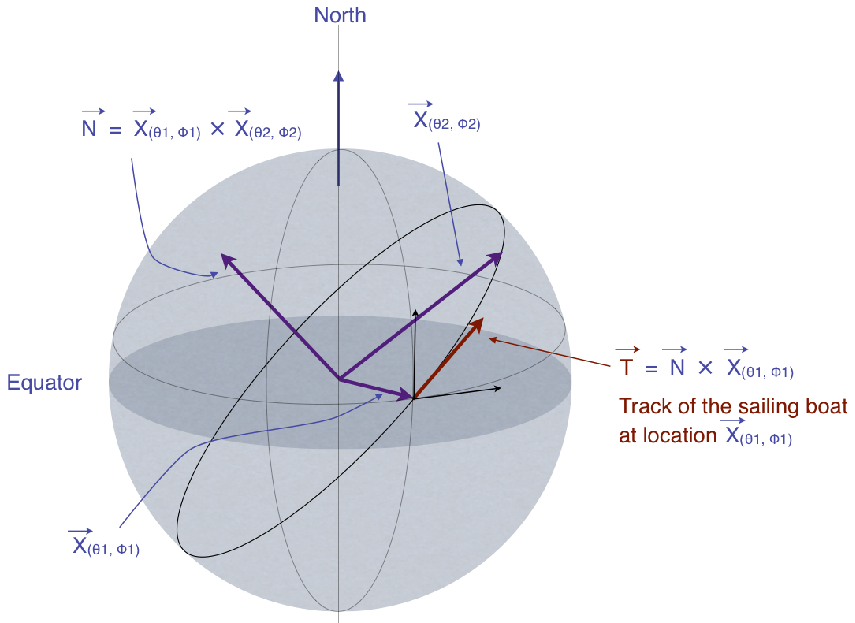
\includegraphics[width=0.8\linewidth]{img/track}
\caption{Berechnung des Kurses}
\label{gridnetConn}
\end{figure}

\subsection{Implementation}
In der Implementation haben wir einen noch einfacheren Ansatz verfolgt:

%\begin{align}
%t = \frac{1}{2} (\frac{2d}{|\mathbf{\overrightarrow{v_{1}}} + \mathbf{\overrightarrow{v_{2}}}|})
%\end{align}

% Siehe letzte SEITE vom PDF "Navigation_Commented_New.pdf"!!!!!
\begin{align}
t = \frac{2d}{\mathbf{s_{1}} + \mathbf{s_{2}}}
\end{align}

t Reisezeit, d Distanz zwischen zwei Punkten, 
$s_{1}$ bzw. $s_{2}$ Schiffsgeschwindigkeit einmal mit Windvektor $v_{1}$ und einmal mit $v_{2}$.

\vspace{0.5cm}
% Im Kapitel 9.1.1 wird es erwähnt... Hier noch ref einfügen!
Würde der Windvektor $v_{2}$ aufgrund von der absoluten Zeit, also in
Bezug zur Uhrzeit, auf das Windfeld des nächsten Zeitabschnitts fallen,
so wird $v_{2}$ mit dem des (zeitlich) nächsten Windfeldes ersetzt.
